% Generated from reviewed lane; compile via book/textbook.tex.
\clearpage

原书 PDF 页 43；印刷页码 30。

\href{source-images/pdf-043.jpeg}{查看原页}

\begin{quote}
本页接上页 2.6 Hermite 插值正文。
\end{quote}

要求高阶导数值也相等。满足这种要求的插值多项式就是 Hermite 插值多项式。下面只讨论函数值与导数值个数相等的情况。设在节点 \(a\leqslant x_0<x_1<\cdots<x_n\leqslant b\) 上，\(y_j=f(x_j),m_j=f'(x_j)\)（\(j=0,1,\cdots,n\)），要求插值多项式 \(H(x)\)，满足条件

\[
H(x_j)=y_j,\quad H'(x_j)=m_j\quad(j=0,1,\cdots,n).\tag{2.6.1}
\]

这里给出的 \(2n+2\) 个条件，可唯一确定一个次数不超过 \(2n+1\) 的多项式

\[H_{2n+1}(x)=H(x),\]

其形式为

\[H_{2n+1}(x)=a_0+a_1x+\cdots+a_{2n+1}x^{2n+1}.\]

如根据条件（2.6.1）来确定 \(2n+2\) 个系数 \(a_0,a_1,\cdots,a_{2n+1}\)，显然非常复杂，因此，仍采用求 Lagrange 插值多项式的基函数方法。先求插值基函数 \(\alpha_j(x)\) 及 \(\beta_j(x)\)（\(j=0,1,\cdots,n\)），共有 \(2n+2\) 个，每一个基函数都是 \(2n+1\) 次多项式，且满足条件

\[
\begin{cases}
\alpha_j(x_k)=\delta_{jk}=\begin{cases}0,&j\ne k,\\1,&j=k,\end{cases}\quad \alpha'_j(x_k)=0\quad(j,k=0,1,\cdots,n),\\
\beta_j(x_k)=0,\quad \beta'_j(x_k)=\delta_{jk}.
\end{cases}\tag{2.6.2}
\]

于是满足条件（2.6.1）的插值多项式 \(H(x)=H_{2n+1}(x)\) 可写成用插值基函数表示的形式，即

\[H_{2n+1}(x)=\sum_{j=0}^{n}[y_j\alpha_j(x)+m_j\beta_j(x)].\tag{2.6.3}\]

由条件（2.6.2），显然有

\[H_{2n+1}(x_k)=y_k,\quad H'_{2n+1}(x_k)=m_k\quad(k=0,1,\cdots,n).\]

下面的问题就是求满足条件（2.6.2）的基函数 \(\alpha_j(x)\) 及 \(\beta_j(x)\)。为此，可利用 Lagrange 插值基函数 \(l_j(x)\)。令

\[\alpha_j(x)=(ax+b)l_j^2(x),\]

其中 \(l_j(x)\) 是式（2.2.10）所表示的基函数。由条件式（2.6.2），有

\[\alpha_j(x_j)=(ax_j+b)l_j^2(x_j)=1,\]

\[\alpha'_j(x_j)=l_j(x_j)[al_j(x_j)+2(ax_j+b)l'_j(x_j)]=0,\]

整理，得

\[\begin{cases}ax_j+b=1,\\a+2l'_j(x_j)=0.\end{cases}\]

解得

\[a=-2l'_j(x_j),\quad b=1+2x_jl'_j(x_j).\]

由于

\[l_j(x)=\frac{(x-x_0)\cdots(x-x_{j-1})(x-x_{j+1})\cdots(x-x_n)}{(x_j-x_0)\cdots(x_j-x_{j-1})(x_j-x_{j+1})\cdots(x_j-x_n)},\]

两端取对数再求导，得

\[l'_j(x_j)=\sum_{\substack{k=0\\k\ne j}}^{n}\frac{1}{x_j-x_k},\]

\begin{quote}
续页：基函数的结果见下一页。
\end{quote}

\clearpage

原书 PDF 页 44；印刷页码 31。

\href{source-images/pdf-044.jpeg}{查看原页}

\begin{quote}
本页接上页 2.6 Hermite 插值正文。
\end{quote}

于是

\[\alpha_j(x)=\left[1-2(x-x_j)\sum_{\substack{k=0\\k\ne j}}^n\frac{1}{x_j-x_k}\right]l_j^2(x).\tag{2.6.4}\]

同理可得

\[\beta_j(x)=(x-x_j)l_j^2(x).\tag{2.6.5}\]

还可证明满足条件（2.6.1）的插值多项式是唯一的。用反证法，假设 \(H_{2n+1}(x)\) 及 \(\overline H_{2n+1}(x)\) 均满足条件（2.6.1），于是

\[\varphi(x)=H_{2n+1}(x)-\overline H_{2n+1}(x)\]

在每个节点 \(x_k\) 上均有二重根，即 \(\varphi(x)\) 有 \(2n+2\) 重根。但 \(\varphi(x)\) 是不高于 \(2n+1\) 次的多项式，故 \(\varphi(x)\equiv0\)。唯一性得证。

仿照 Lagrange 插值余项的证明方法，若 \(f(x)\) 在 \((a,b)\) 内的 \(2n+2\) 阶导数存在，则其插值余项

\[R(x)=f(x)-H_{2n+1}(x)=\frac{f^{(2n+2)}(\xi)}{(2n+2)!}\omega_{n+1}^2(x),\tag{2.6.6}\]

其中 \(\xi\in(a,b)\) 且与 \(x\) 有关。具体证明请读者自行完成。

作为带导数插值多项式（2.6.3）的重要特例是 \(n=1\) 的情形。这时可取节点为 \(x_k\) 及 \(x_{k+1}\)，插值多项式为 \(H_3(x)\)，满足条件

\[\begin{cases}
H_3(x_k)=y_k,\quad H_3(x_{k+1})=y_{k+1},\\
H'_3(x_k)=m_k,\quad H'_3(x_{k+1})=m_{k+1}.
\end{cases}\tag{2.6.7}\]

相应的插值基函数为 \(\alpha_k(x),\alpha_{k+1}(x),\beta_k(x),\beta_{k+1}(x)\)，它们满足条件

\[\begin{gathered}
\alpha_k(x_k)=1,\quad\alpha_k(x_{k+1})=0,\quad\alpha'_k(x_k)=\alpha'_k(x_{k+1})=0,\\
\alpha_{k+1}(x_k)=0,\quad\alpha_{k+1}(x_{k+1})=1,\\
\alpha'_{k+1}(x_k)=\alpha'_{k+1}(x_{k+1})=0,\quad\beta_k(x_k)=\beta_k(x_{k+1})=0,\\
\beta'_k(x_k)=1,\quad\beta'_k(x_{k+1})=0,\quad\beta_{k+1}(x_k)=\beta_{k+1}(x_{k+1})=0,\\
\beta'_{k+1}(x_k)=0,\quad\beta'_{k+1}(x_{k+1})=1.
\end{gathered}\]

根据式（2.6.4）及式（2.6.5）的一般表达式，可得

\[\begin{cases}
\displaystyle\alpha_k(x)=\left(1+2\frac{x-x_k}{x_{k+1}-x_k}\right)\left(\frac{x-x_{k+1}}{x_k-x_{k+1}}\right)^2,\\[6pt]
\displaystyle\alpha_{k+1}(x)=\left(1+2\frac{x-x_{k+1}}{x_k-x_{k+1}}\right)\left(\frac{x-x_k}{x_{k+1}-x_k}\right)^2;
\end{cases}\tag{2.6.8}\]

\[\begin{cases}
\displaystyle\beta_k(x)=(x-x_k)\left(\frac{x-x_{k+1}}{x_k-x_{k+1}}\right)^2,\\[6pt]
\displaystyle\beta_{k+1}(x)=(x-x_{k+1})\left(\frac{x-x_k}{x_{k+1}-x_k}\right)^2.
\end{cases}\tag{2.6.9}\]

于是满足条件（2.6.7）的插值多项式是

\[H_3(x)=y_k\alpha_k(x)+y_{k+1}\alpha_{k+1}(x)+m_k\beta_k(x)+m_{k+1}\beta_{k+1}(x),\tag{2.6.10}\]

其余项 \(R_3(x)=f(x)-H_3(x)\)，由式（2.6.6）得

\begin{quote}
续页：余项公式见下一页。
\end{quote}

\clearpage

原书 PDF 页 45；印刷页码 32。

\href{source-images/pdf-045.jpeg}{查看原页}

\begin{quote}
本页接上页 2.6 Hermite 插值正文。
\end{quote}

\[R_3(x)=\frac{1}{4!}f^{(4)}(\xi)(x-x_k)^2(x-x_{k+1})^2.\]

\textbf{例 2.5}　求满足 \(P(x_j)=f(x_j)\)（\(j=0,1,2\)）及 \(P'(x_1)=f'(x_1)\) 的插值多项式及其余项表达式。

\textbf{解}　由给定条件，可确定次数不超过 3 的插值多项式。由于此多项式通过点 \((x_0,f(x_0)),(x_1,f(x_1))\) 及 \((x_2,f(x_2))\)，故其形式为

\[\begin{aligned}
P(x)={}&f(x_0)+f[x_0,x_1](x-x_0)+f[x_0,x_1,x_2](x-x_0)(x-x_1)\\
&+A(x-x_0)(x-x_1)(x-x_2),
\end{aligned}\]

其中 \(A\) 为待定常数，可由条件 \(P'(x_1)=f'(x_1)\) 确定，通过计算可得

\[A=\frac{f'(x_1)-f[x_0,x_1]-(x_1-x_0)f[x_0,x_1,x_2]}{(x_1-x_0)(x_1-x_2)}.\]

为了求出余项 \(R(x)=f(x)-P(x)\) 的表达式，可设

\[R(x)=f(x)-P(x)=K(x)(x-x_0)(x-x_1)^2(x-x_2),\]

其中 \(K(x)\) 为待定函数。构造

\[\varphi(t)=f(t)-P(t)-K(x)(t-x_0)(t-x_1)^2(t-x_2).\]

显然 \(\varphi(x_j)=0\)（\(j=0,1,2\)），且 \(\varphi'(x_1)=0,\varphi(x)=0\)，故 \(\varphi(t)\) 在 \((a,b)\) 内有五个零点（重根算两个）。反复应用 Rolle 定理得，\(\varphi^{(4)}(t)\) 在 \((a,b)\) 内至少有一个零点 \(\xi\)，故

\[\varphi^{(4)}(\xi)=f^{(4)}(\xi)-4!K(x)=0,\]

于是 \(K(x)=f^{(4)}(\xi)/4!\)，余项表达式为

\[R(x)=f^{(4)}(\xi)(x-x_0)(x-x_1)^2(x-x_2)/4!,\tag{2.6.11}\]

其中 \(\xi\) 位于 \(x_0,x_1,x_2\) 和 \(x\) 所界定的范围内。

\subsection{2.7 分段低次插值}\label{ch02b-ux5206ux6bb5ux4f4eux6b21ux63d2ux503c}

\subsubsection{2.7.1 多项式插值的问题}\label{ch02b-ux591aux9879ux5f0fux63d2ux503cux7684ux95eeux9898}

根据区间 \([a,b]\) 上给出的节点构造插值多项式 \(L_n(x)\) 近似 \(f(x)\) 时，人们往往认为 \(L_n(x)\) 的次数 \(n\) 越高逼近 \(f(x)\) 的精度越好，但实际上并非如此。这是因为，对于任意的插值节点，当 \(n\to\infty\) 时，\(L_n(x)\) 不一定收敛到 \(f(x)\)。20 世纪初 Runge 就给出了一个等距节点插值多项式 \(L_n(x)\) 不收敛到 \(f(x)\) 的例子：考察函数 \(f(x)=1/(1+x^2)\)，它在 \([-5,5]\) 上各阶导数均存在，但在 \([-5,5]\) 上取 \(n+1\) 个等距节点

\[x_k=-5+10\frac{k}{n}\quad(k=0,1,\cdots,n)\]

所构造的 Lagrange 插值多项式

\begin{quote}
续页：该多项式和 Runge 现象见下一页。
\end{quote}

\clearpage

原书 PDF 页 46；印刷页码 33。

\href{source-images/pdf-046.jpeg}{查看原页}

\begin{quote}
本页接上页 2.7.1 正文。
\end{quote}

\[L_n(x)=\sum_{j=0}^n\frac{1}{1+x_j^2}\frac{\omega_{n+1}(x)}{(x-x_j)\omega'_{n+1}(x_j)}\]

当 \(n\to\infty\) 时只在 \(|x|\leqslant3.63\) 内收敛，而在这区间外是发散的。

下面取 \(n=10\)，根据计算画出 \(y=L_{10}(x)\) 及 \(y=1/(1+x^2)\) 在 \([-5,5]\) 上的图形，如图 2.5 所示。

从图 2.5 可看到，在 \(x=\pm5\) 附近 \(L_{10}(x)\) 与 \(f(x)=1/(1+x^2)\) 偏离很远，例如，\(L_{10}(4.8)=1.804\,38,f(4.8)=0.041\,60\)。这说明用高次插值多项式 \(L_n(x)\) 近似 \(f(x)\) 效果并不好，因而通常不用高次插值，而用低次插值。从该例看到，如果把 \(y=1/(1+x^2)\) 在节点 \(x=0,\pm1,\pm2,\pm3,\pm4,\pm5\) 处用折线连起来，显然比 \(L_{10}(x)\) 逼近 \(f(x)\) 好得多。这正是下面要讨论的分段低次插值的出发点。

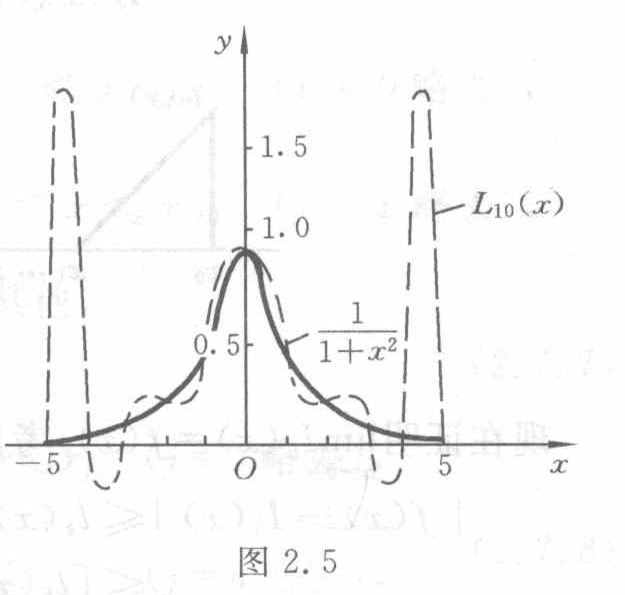
\includegraphics[width=0.85\linewidth,height=\textheight,keepaspectratio,alt={图 2.5（原图裁切）}]{verified/assets/ch02b/figure-2-5.png}

\begin{quote}
图 2.5（原图）：横轴 \(x\)，纵轴 \(y\)，原点 \(O\)；横轴标有 \(-5,5\)，纵轴标有 \(0.5,1.0,1.5\)。两条曲线标签为 \(L_{10}(x)\) 与 \(\frac{1}{1+x^2}\)。虚线插值曲线在两端附近出现明显振荡。
\end{quote}

\subsubsection{2.7.2 分段线性插值}\label{ch02b-ux5206ux6bb5ux7ebfux6027ux63d2ux503c}

所谓分段线性插值，就是将插值点用折线段连接起来逼近 \(f(x)\)。设已知节点 \(a=x_0<x_1<\cdots<x_n=b\) 上的函数值 \(f_0,f_1,\cdots,f_n\)，记 \(h_k=x_{k+1}-x_k,h=\max_k h_k\)。称 \(I_h(x)\) 为分段线性插值函数，如果满足：

（1）记 \(I_h(x)\in C[a,b]\)；

（2）\(I_h(x_k)=f_k\)（\(k=0,1,\cdots,n\)）；

（3）\(I_h(x)\) 在每个区间 \([x_k,x_{k+1}]\) 上是线性函数，

则由定义可知，\(I_h(x)\) 在每个小区间 \([x_k,x_{k+1}]\) 上可表示为

\[I_h(x)=\frac{x-x_{k+1}}{x_k-x_{k+1}}f_k+\frac{x-x_k}{x_{k+1}-x_k}f_{k+1}\quad(x_k\leqslant x\leqslant x_{k+1}).\tag{2.7.1}\]

若用插值基函数表示，则 \(I_h(x)\) 在整个区间 \([a,b]\) 上可表示为

\[I_h(x)=\sum_{j=0}^n f_jl_j(x),\tag{2.7.2}\]

其中基函数 \(l_j(x)\) 满足条件 \(l_j(x_k)=\delta_{jk}\)（\(j,k=0,1,\cdots,n\)），其形式是

\[l_j(x)=\begin{cases}
\displaystyle\frac{x-x_{j-1}}{x_j-x_{j-1}},&x_{j-1}\leqslant x\leqslant x_j\quad(j=0\text{ 略去}),\\[6pt]
\displaystyle\frac{x_j-x_{j+1}}{x-x_{j+1}},&x_j\leqslant x\leqslant x_{j+1}\quad(j=n\text{ 略去}),\\[6pt]
0,&x\in[a,b],\quad x\notin[x_{j-1},x_{j+1}].
\end{cases}\tag{2.7.3}\]

分段线性插值基函数 \(l_j(x)\) 只在 \(x_j\) 附近不为零，在其他地方均为零，这种性质称为\textbf{局部非零性质}，如图 2.6 所示。当 \(x\in[x_k,x_{k+1}]\) 时，

\begin{quote}
续页：基函数恒等式和图 2.6 见下一页。
\end{quote}

\begin{quote}
\textbf{校注（agent 补充；原书疑误）}：式（2.7.3）第二分支原扫描确为 \(\frac{x_j-x_{j+1}}{x-x_{j+1}}\)，此处已原样保留，参见\href{verified/assets/ch02b/pdf-046-eq-2-7-3-detail.png}{原式放大裁图}。该式在 \(x=x_{j+1}\) 处分母为零，与本页分段线性、连续性及 \(l_j(x_{j+1})=0\) 的条件矛盾。按这些条件，第二分支应为 \(\frac{x-x_{j+1}}{x_j-x_{j+1}}\)。这属于原书疑误，区别于 OCR 另将分母误识为 \(x_j-x_{j+1}\)。
\end{quote}

\clearpage

原书 PDF 页 47；印刷页码 34。

\href{source-images/pdf-047.jpeg}{查看原页}

\begin{quote}
本页接上页 2.7.2 正文。
\end{quote}

\[1=\sum_{j=0}^nl_j(x)=l_k(x)+l_{k+1}(x),\quad f(x)=[l_k(x)+l_{k+1}(x)]f(x).\]

另一方面，这时

\[I_h(x)=f_kl_k(x)+f_{k+1}l_{k+1}(x).\]

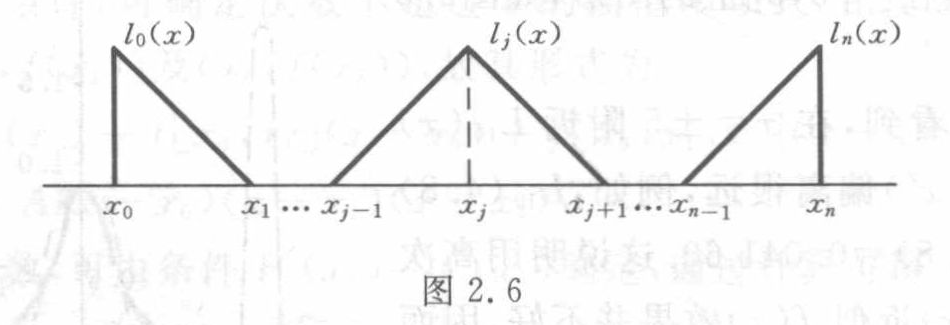
\includegraphics[width=0.85\linewidth,height=\textheight,keepaspectratio,alt={图 2.6（原图裁切）}]{verified/assets/ch02b/figure-2-6.png}

\begin{quote}
图 2.6（原图）：分段线性插值基函数的局部非零形状。左端 \(l_0(x)\) 在 \(x_0\) 达到峰值并线性降到 \(x_1\)；内部 \(l_j(x)\) 在 \(x_{j-1},x_{j+1}\) 为零，在 \(x_j\) 达到峰值；右端 \(l_n(x)\) 从 \(x_{n-1}\) 线性升到 \(x_n\)。全部原图标签为 \(l_0(x),l_j(x),l_n(x),x_0,x_1,\cdots,x_{j-1},x_j,x_{j+1},\cdots,x_{n-1},x_n\)；峰值未标数字。
\end{quote}

现在证明 \(\lim_{h\to0}I_h(x)=f(x)\)。考虑

\[\begin{aligned}
|f(x)-I_h(x)|&\leqslant l_k(x)|f(x)-f_k|+l_{k+1}(x)|f(x)-f_{k+1}|\\
&\leqslant[l_k(x)+l_{k+1}(x)]\omega(h_k)\\
&=\omega(h_k)\leqslant\omega(h),
\end{aligned}\tag{2.7.4}\]

这里 \(\omega(h)\) 是函数 \(f(x)\) 在区间 \([a,b]\) 上的\textbf{连续模}，即对于任意两点 \(x',x''\in[a,b]\)，只要 \(|x'-x''|\leqslant h\)，就有

\[|f(x')-f(x'')|\leqslant\omega(h),\]

称 \(\omega(h)\) 为 \(f(x)\) 在 \([a,b]\) 上的连续模，当 \(f(x)\in C[a,b]\) 时，就有 \(\lim_{h\to0}\omega(h)=0\)。

由前式可知，当 \(x\in[a,b]\) 时有 \(\max_{a\leqslant x\leqslant b}|f(x)-I_h(x)|\leqslant\omega(h)\)，因此，只要 \(f(x)\in C[a,b]\)，就有 \(\lim_{h\to0}I_h(x)=f(x)\) 在 \([a,b]\) 上一致成立，故 \(I_h(x)\) 在 \([a,b]\) 上一致收敛到 \(f(x)\)。

\subsubsection{2.7.3 分段三次 Hermite 插值}\label{ch02b-ux5206ux6bb5ux4e09ux6b21-hermite-ux63d2ux503c}

分段线性插值函数 \(I_h(x)\) 的导数是间断的，若在节点 \(x_k\)（\(k=0,1,\cdots,n\)）上除已知函数值 \(f_k\) 外还给出导数值 \(f'_k=m_k\)（\(k=0,1,\cdots,n\)），就可构造一个导数连续的分段插值函数 \(I_h(x)\)，它满足如下条件：

（1）\(I_h(x)\in C^1[a,b]\)（\(C^1[a,b]\) 代表区间 \([a,b]\) 上一阶导数连续的函数集合）；

（2）\(I_h(x_k)=f_k,I'_h(x_k)=f'_k\)（\(k=0,1,\cdots,n\)）；

（3）\(I_h(x)\) 在每个小区间 \([x_k,x_{k+1}]\) 上是三次多项式。

根据两点三次插值多项式（2.6.10）可知，\(I_h(x)\) 在区间 \([x_k,x_{k+1}]\) 上的表达式为

\[\begin{aligned}
I_h(x)={}&\left(\frac{x-x_{k+1}}{x_k-x_{k+1}}\right)^2\left(1+2\frac{x-x_k}{x_{k+1}-x_k}\right)f_k+\left(\frac{x-x_k}{x_{k+1}-x_k}\right)^2\left(1+2\frac{x-x_{k+1}}{x_k-x_{k+1}}\right)f_{k+1}\\
&+\left(\frac{x-x_{k+1}}{x_k-x_{k+1}}\right)^2(x-x_k)f'_k+\left(\frac{x-x_k}{x_{k+1}-x_k}\right)^2(x-x_{k+1})f'_{k+1}.
\end{aligned}\tag{2.7.5}\]

若在整个区间 \([a,b]\) 上定义一组分段三次插值基函数 \(\alpha_j(x)\) 及 \(\beta_j(x)\)（\(j=0,\)

\begin{quote}
续页：上句的下标范围及公式在下一页续完。
\end{quote}

\clearpage

原书 PDF 页 48；印刷页码 35。

\href{source-images/pdf-048.jpeg}{查看原页}

\begin{quote}
本页接上页 2.7.3 正文；开头续完下标范围。
\end{quote}

\(1,\cdots,n\)），则 \(I_h(x)\) 可表示为

\[I_h(x)=\sum_{j=0}^n[f_j\alpha_j(x)+f'_j\beta_j(x)],\tag{2.7.6}\]

其中 \(\alpha_j(x),\beta_j(x)\) 依式（2.6.8）、式（2.6.9）分别表示为

\[\alpha_j(x)=\begin{cases}
\displaystyle\left(\frac{x-x_{j-1}}{x_j-x_{j-1}}\right)^2\left(1+2\frac{x-x_j}{x_{j-1}-x_j}\right),&x_{j-1}\leqslant x\leqslant x_j\quad(j=0\text{ 略去}),\\[6pt]
\displaystyle\left(\frac{x-x_{j+1}}{x_j-x_{j+1}}\right)^2\left(1+2\frac{x-x_j}{x_{j+1}-x_j}\right),&x_j\leqslant x\leqslant x_{j+1}\quad(j=n\text{ 略去}),\\[6pt]
0,&\text{其他},
\end{cases}\tag{2.7.7}\]

\[\beta_j(x)=\begin{cases}
\displaystyle\left(\frac{x-x_{j-1}}{x_j-x_{j-1}}\right)^2(x-x_j),&x_{j-1}\leqslant x\leqslant x_j\quad(j=0\text{ 略去}),\\[6pt]
\displaystyle\left(\frac{x-x_{j+1}}{x_j-x_{j+1}}\right)^2(x-x_j),&x_j\leqslant x\leqslant x_{j+1}\quad(j=n\text{ 略去}),\\[6pt]
0,&\text{其他}.
\end{cases}\tag{2.7.8}\]

由于 \(\alpha_j(x),\beta_j(x)\) 的局部非零性质，当 \(x\in[x_k,x_{k+1}]\) 时，只有 \(\alpha_k(x),\alpha_{k+1}(x),\beta_k(x),\beta_{k+1}(x)\) 不为零，于是式（2.7.6）的 \(I_h(x)\) 可表示为

\[I_h(x)=f_k\alpha_k(x)+f_{k+1}\alpha_{k+1}(x)+f'_k\beta_k(x)+f'_{k+1}\beta_{k+1}(x)\quad(x_k\leqslant x\leqslant x_{k+1}).\tag{2.7.9}\]

为了研究 \(I_h(x)\) 的收敛性，由式（2.7.7）及式（2.7.8）直接得估计式

\[0\leqslant\alpha_j(x)\leqslant1,\tag{2.7.10}\]

\[\begin{cases}
\displaystyle|\beta_k(x)|\leqslant\frac{4}{27}h_k,\\[6pt]
\displaystyle|\beta_{k+1}(x)|\leqslant\frac{4}{27}h_k.
\end{cases}\tag{2.7.11}\]

此外，当 \(f(x)\) 是分段三次多项式时，\(f(x)\) 的插值多项式 \(I_h(x)\) 就是它本身。例如，当 \(f(x)=1\) 时就有 \(\sum_{j=0}^n\alpha_j(x)=1\)。当 \(x\in[x_k,x_{k+1}]\) 时，得

\[\alpha_k(x)+\alpha_{k+1}(x)=1.\tag{2.7.12}\]

由式（2.7.9）～（2.7.12），当 \(x\in[x_k,x_{k+1}]\) 时还可得

\[\begin{aligned}
|f(x)-I_h(x)|&\leqslant\alpha_k(x)|f(x)-f_k|+\alpha_{k+1}(x)|f(x)-f_{k+1}|\\
&\quad+\frac{4}{27}h_k[|f'_k|+|f'_{k+1}|]\\
&\leqslant[\alpha_k(x)+\alpha_{k+1}(x)]\omega(h)+\frac{8}{27}h\max\{|f'_k|,|f'_{k+1}|\},
\end{aligned}\]

\[|f(x)-I_h(x)|\leqslant\omega(h)+\frac{8}{27}h\max_{0\leqslant k\leqslant n}|f'_k|\tag{2.7.13}\]

对于 \(x\in[a,b]\) 成立，其中 \(\omega(h)\) 是 \(f(x)\) 在 \([a,b]\) 上的连续模。因此，当 \(f(x)\in C[a,b]\)

\begin{quote}
续页：收敛性论述在下一页续完。
\end{quote}

\clearpage

原书 PDF 页 49；印刷页码 36。

\href{source-images/pdf-049.jpeg}{查看原页}

\begin{quote}
本页接上页 2.7.3 正文。
\end{quote}

时，

\[\lim_{h\to0}I_h(x)=f(x).\]

这就证明了 \(I_h(x)\) 在 \([a,b]\) 上一致收敛到 \(f(x)\)。

\subsection{2.8 三次样条插值}\label{ch02b-ux4e09ux6b21ux6837ux6761ux63d2ux503c}

上面讨论的分段低次插值函数都有一致收敛性，但光滑性较差，对于像高速飞机的机翼、船体放样等的型值线，往往要求有二阶光滑度，即有二阶连续导数。早期工程师制图时，把富有弹性的细长木条（所谓样条）用压铁固定在样点上，在其他地方让它自由弯曲，然后画下长条的曲线，称为样条曲线。它实际上是由分段三次曲线并接而成，在连接点即样点上要求二阶导数连续，从数学上加以概括就得到数学样条这一概念。下面讨论最常用的三次样条函数。

\subsubsection{2.8.1 三次样条函数}\label{ch02b-ux4e09ux6b21ux6837ux6761ux51fdux6570}

\textbf{定义 2.5}　若函数 \(S(x)\in C^2[a,b]\)，且在每个小区间 \([x_j,x_{j+1}]\) 上是三次多项式，其中 \(a=x_0<x_1<\cdots<x_n=b\) 是给定节点，则称 \(S(x)\) 是节点 \(x_0,x_1,\cdots,x_n\) 上的\textbf{三次样条函数}。若在节点 \(x_j\) 上给定函数值 \(y_j=f(x_j)\)（\(j=0,1,\cdots,n\)），且

\[S(x_j)=y_j\quad(j=0,1,\cdots,n)\tag{2.8.1}\]

成立，则称 \(S(x)\) 为\textbf{三次样条插值函数}。

从定义知，要求出 \(S(x)\)，在每个小区间 \([x_j,x_{j+1}]\) 上要确定 4 个待定系数，共有 \(n\) 个小区间，故应确定 \(4n\) 个参数。根据 \(S(x)\) 在 \([a,b]\) 上二阶导数连续，在节点 \(x_j\)（\(j=1,2,\cdots,n-1\)）处应满足连续性条件

\[\begin{gathered}
S(x_j-0)=S(x_j+0),\quad S'(x_j-0)=S'(x_j+0),\\
S''(x_j-0)=S''(x_j+0),
\end{gathered}\tag{2.8.2}\]

共有 \(3n-3\) 个条件，再加上 \(S(x)\) 满足插值条件（2.8.1），共有 \(4n-2\) 个条件，因此还需要 2 个条件才能确定 \(S(x)\)。通常可在区间 \([a,b]\) 端点 \(a=x_0,b=x_n\) 上各加一个条件（称为\textbf{边界条件}），边界条件可根据实际问题的要求给定。常见的有以下三种：

（1）已知两端的一阶导数值，即

\[\begin{cases}S'(x_0)=f'_0,\\S'(x_n)=f'_n.\end{cases}\tag{2.8.3}\]

（2）两端的二阶导数已知，即

\[\begin{cases}S''(x_0)=f''_0,\\S''(x_n)=f''_n.\end{cases}\tag{2.8.4}\]

特殊情况下的边界条件

\begin{quote}
续页：自然边界条件及第三类边界条件见下一页。
\end{quote}

\begin{quote}
\textbf{校注（agent 补充；原书论证条件疑漏）}：本页开头承接上一页``当 \(f(x)\in C[a,b]\) 时''即宣称分段三次 Hermite 插值一致收敛，原文已保留。由（2.7.13）实际还需控制 \(h\max_k|f'_k|\to0\)；仅有连续性既不保证节点导数存在，也不能控制随加密节点变化的导数值。比如加上 \(f\in C^1[a,b]\) 就足以使节点导数一致有界，从该估计推出结论。本注是对原文论证条件的补充，不属于教材正文。
\end{quote}

\clearpage

原书 PDF 页 50；印刷页码 37。

\href{source-images/pdf-050.jpeg}{查看原页}

\begin{quote}
本页接上页 2.8.1 正文。
\end{quote}

\[S''(x_0)=S''(x_n)=0\tag{2.8.4'}\]

称为\textbf{自然边界条件}。

（3）当 \(f(x)\) 是以 \(x_n-x_0\) 为周期的周期函数时，则要求 \(S(x)\) 也是周期函数，这时边界条件应满足

\[\begin{cases}
S(x_0+0)=S(x_n-0),\\
S'(x_0+0)=S'(x_n-0),\\
S''(x_0+0)=S''(x_n-0),
\end{cases}\tag{2.8.5}\]

而此时式（2.8.1）中 \(y_0=y_n\)。这样确定的样条函数 \(S(x)\) 称为\textbf{周期样条函数}。

\subsubsection{2.8.2 三转角方程}\label{ch02b-ux4e09ux8f6cux89d2ux65b9ux7a0b}

现在构造满足条件（2.8.1）及加上相应边界条件的三次样条函数 \(S(x)\) 的表达式。若假定 \(S'(x)\) 在节点 \(x_j\) 处的值为 \(S'(x_j)=m_j\)（\(j=0,1,\cdots,n\)），再由式（2.8.1），则由分段三次 Hermite 插值式（2.7.6）可得

\[S(x)=\sum_{j=0}^n[y_j\alpha_j(x)+m_j\beta_j(x)],\tag{2.8.6}\]

其中 \(\alpha_j(x),\beta_j(x)\) 是插值基函数，由式（2.7.7）、式（2.7.8）表示。显然，表达式（2.8.6）中 \(S(x)\) 及 \(S'(x)\) 在整个区间 \([a,b]\) 上连续，且满足式（2.8.1）；然而在式（2.8.6）中 \(m_j\)（\(j=0,1,\cdots,n\)）是未知的，它可利用式（2.8.2）

\[S''(x_j-0)=S''(x_j+0)\quad(j=1,\cdots,n-1)\]

及边界条件（2.8.3）（也可以是其他边界条件）来确定。为了求出 \(m_j\)，下面考虑 \(S(x)\) 在 \([x_j,x_{j+1}]\) 上的表达式

\[\begin{aligned}
S(x)={}&\frac{(x-x_{j+1})^2[h_j+2(x-x_j)]}{h_j^3}y_j+\frac{(x-x_j)^2[h_j+2(x_{j+1}-x)]}{h_j^3}y_{j+1}\\
&+\frac{(x-x_{j+1})^2(x-x_j)}{h_j^2}m_j+\frac{(x-x_j)^2(x-x_{j+1})}{h_j^2}m_{j+1},
\end{aligned}\tag{2.8.7}\]

这里 \(h_j=x_{j+1}-x_j\)。对 \(S(x)\) 求二阶导数，得

\[\begin{aligned}
S''(x)={}&\frac{6x-2x_j-4x_{j+1}}{h_j^2}m_j+\frac{6x-4x_j-2x_{j+1}}{h_j^2}m_{j+1}\\
&+\frac{6(x_j+x_{j+1}-2x)}{h_j^3}(y_{j+1}-y_j),
\end{aligned}\]

于是

\[S''(x_j+0)=-\frac4{h_j}m_j-\frac2{h_j}m_{j+1}+\frac6{h_j^2}(y_{j+1}-y_j).\]

同理，可得 \(S''(x)\) 在区间 \([x_{j-1},x_j]\) 上的表达式

\[\begin{aligned}
S''(x)={}&\frac{6x-2x_{j-1}-4x_j}{h_{j-1}^2}m_{j-1}+\frac{6x-4x_{j-1}-2x_j}{h_{j-1}^2}m_j\\
&+\frac{6(x_{j-1}+x_j-2x)}{h_{j-1}^2}(y_j-y_{j-1})
\end{aligned}\]

\begin{quote}
续页：左侧二阶导数在下一页继续。
\end{quote}

\begin{quote}
\textbf{校注（agent 补充；原书疑误）}：本页末式第三项的分母在原扫描中为 \(h_{j-1}^2\)，上面原样保留，参见\href{verified/assets/ch02b/pdf-050-second-derivative-detail.png}{原式放大裁图}。由同页前一个区间的 \(S''(x)\) 公式换下标，第三项分母应为 \(h_{j-1}^3\)；这样代入 \(x=x_j\) 才得到下一页的 \(-6(y_j-y_{j-1})/h_{j-1}^2\)。这是原书幂次疑误；OCR 还漏掉了多个 \(j-1\) 下标，已按图补回。
\end{quote}

\clearpage

原书 PDF 页 51；印刷页码 38。

\href{source-images/pdf-051.jpeg}{查看原页}

\begin{quote}
本页接上页 2.8.2 正文。
\end{quote}

及

\[S''(x_j-0)=\frac2{h_{j-1}}m_{j-1}+\frac4{h_{j-1}}m_j-\frac6{h_{j-1}^2}(y_j-y_{j-1}).\]

由条件 \(S''(x_j+0)=S''(x_j-0)\)（\(j=1,2,\cdots,n-1\)），可得

\[\begin{aligned}
&\frac1{h_{j-1}}m_{j-1}+2\left(\frac1{h_{j-1}}+\frac1{h_j}\right)m_j+\frac1{h_j}m_{j+1}\\
&\qquad=3\left(\frac{y_{j+1}-y_j}{h_j^2}+\frac{y_j-y_{j-1}}{h_{j-1}^2}\right)\quad(j=1,2,\cdots,n-1),
\end{aligned}\tag{2.8.8}\]

用 \(\frac1{h_{j-1}}+\frac1{h_j}\) 除全式，并注意 \(y_j=f_j,\frac{y_{j+1}-y_j}{h_j}=f[x_j,x_{j+1}]\)，方程（2.8.8）可简化为

\[\lambda_jm_{j-1}+2m_j+\mu_jm_{j+1}=g_j\quad(j=1,2,\cdots,n-1),\tag{2.8.9}\]

其中

\[\lambda_j=\frac{h_j}{h_{j-1}+h_j},\quad\mu_j=\frac{h_{j-1}}{h_{j-1}+h_j}\quad(j=1,2,\cdots,n-1),\tag{2.8.10}\]

\[g_j=3(\lambda_jf[x_{j-1},x_j]+\mu_jf[x_j,x_{j+1}])\quad(j=1,2,\cdots,n-1).\tag{2.8.11}\]

方程（2.8.9）是关于未知数 \(m_0,m_1,\cdots,m_n\) 的 \(n-1\) 个方程，若加上已知条件（2.8.3）：\(m_0=f'_0\) 则 \(m_n=f'_n\)，那么方程（2.8.9）为只含 \(m_1,\cdots,m_{n-1}\) 的 \(n-1\) 个方程，写成矩阵形式便是

\[\begin{pmatrix}
2&\mu_1&0&\cdots&\cdots&0\\
\lambda_2&2&\mu_2&\ddots&&\vdots\\
0&\lambda_3&2&\mu_3&\ddots&\vdots\\
\vdots&\ddots&\ddots&\ddots&\ddots&0\\
0&&\ddots&\lambda_{n-2}&2&\mu_{n-2}\\
0&\cdots&\cdots&0&\lambda_{n-1}&2
\end{pmatrix}
\begin{pmatrix}m_1\\m_2\\m_3\\\vdots\\m_{n-2}\\m_{n-1}\end{pmatrix}
=\begin{pmatrix}g_1-\lambda_1f'_0\\g_2\\g_3\\\vdots\\g_{n-2}\\g_{n-1}-\mu_{n-1}f'_n\end{pmatrix}.\tag{2.8.12}\]

如果边界条件为式（2.8.4），则

\[\begin{cases}
\displaystyle2m_0+m_1=3f[x_0,x_1]-\frac{h_0}2f''_0=g_0,\\[6pt]
\displaystyle m_{n-1}+2m_n=3f[x_{n-1},x_n]+\frac{h_{n-1}}2f''_n=g_n.
\end{cases}\tag{2.8.13}\]

如果边界条件为式（2.8.4）′，则

\[\begin{cases}
2m_0+m_1=3f[x_0,x_1]=g_0,\\
m_{n-1}+2m_n=3f[x_{n-1},x_n]=g_n.
\end{cases}\tag{2.8.13'}\]

于是，式（2.8.9）与式（2.8.13）或式（2.8.13）′合并后用矩阵形式表示为

\[\begin{pmatrix}
2&1&0&\cdots&\cdots&0\\
\lambda_1&2&\mu_1&\ddots&&\vdots\\
0&\lambda_2&2&\mu_2&\ddots&\vdots\\
\vdots&\ddots&\ddots&\ddots&\ddots&0\\
\vdots&&\ddots&\lambda_{n-1}&2&\mu_{n-1}\\
0&\cdots&\cdots&0&1&2
\end{pmatrix}
\begin{pmatrix}m_0\\m_1\\m_2\\\vdots\\m_{n-1}\\m_n\end{pmatrix}
=\begin{pmatrix}g_0\\g_1\\g_2\\\vdots\\g_{n-1}\\g_n\end{pmatrix}.\tag{2.8.14}\]

\clearpage

原书 PDF 页 52；印刷页码 39。

\href{source-images/pdf-052.jpeg}{查看原页}

\begin{quote}
本页接上页 2.8.2 正文。
\end{quote}

如果边界条件为周期性条件式（2.8.5），则

\[m_0=m_n,\]

\[\frac1{h_0}m_1+\frac1{h_{n-1}}m_{n-1}+2\left(\frac1{h_0}+\frac1{h_{n-1}}\right)m_n=\frac3{h_0}f[x_0,x_1]+\frac3{h_{n-1}}f[x_{n-1},x_n],\]

化简为

\[\mu_nm_1+\lambda_nm_{n-1}+2m_n=g_n,\]

\[\mu_n=\frac{h_{n-1}}{h_0+h_{n-1}},\quad\lambda_n=\frac{h_{n-1}}{h_0+h_{n-1}},\]

\[g_n=3(\mu_nf[x_0,x_1]+\lambda_nf[x_{n-1},x_n]).\]

与式（2.8.9）合并，用矩阵形式表示为

\[\begin{pmatrix}
2&\mu_1&0&\cdots&0\\
\lambda_2&2&\mu_2&\ddots&\vdots\\
0&\lambda_3&\ddots&\ddots&0\\
\vdots&\ddots&\ddots&2&\mu_{n-1}\\
0&\cdots&0&\lambda_n&2
\end{pmatrix}
\begin{pmatrix}m_1\\m_2\\\vdots\\m_{n-1}\\m_n\end{pmatrix}
=\begin{pmatrix}g_1\\g_2\\\vdots\\g_{n-1}\\g_n\end{pmatrix}.\tag{2.8.15}\]

这里得到的方程组（2.8.12）、（2.8.14）及式（2.8.15）中，每个方程都联系三个 \(m_j\)，\(m_j\) 在力学上解释为细梁在 \(x_j\) 截面处的转角，故称之为\textbf{三转角方程}。这些方程系数矩阵对角元素均为 2，非对角元素 \(\mu_j+\lambda_j=1\)，故系数矩阵具有强对角优势，方程组（2.8.12）、（2.8.14）及（2.8.15）都有唯一解，可用追赶法求得解 \(m_j\)（\(j=0,1,\cdots,n\)），从而得到 \(S(x)\)。关于线性方程组的解法见本书第 7 章。

\subsubsection{2.8.3 三弯矩方程}\label{ch02b-ux4e09ux5f2fux77e9ux65b9ux7a0b}

三次样条插值函数 \(S(x)\) 可以有多种表达方法，有时用二阶导数值 \(S''(x_j)=M_j\)（\(j=0,1,\cdots,n\)）表示使用起来更方便。\(M_j\) 在力学上解释为细梁在 \(x_j\) 截面处的弯矩，并且得到的弯矩与相邻两个弯矩有关，故称之为\textbf{三弯矩方程}。

由于 \(S(x)\) 在区间 \([x_j,x_{j+1}]\) 上是三次多项式，故 \(S''(x)\) 在 \([x_j,x_{j+1}]\) 上是线性函数，可表示为

\[S''(x)=M_j\frac{x_{j+1}-x}{h_j}+M_{j+1}\frac{x-x_j}{h_j}.\tag{2.8.16}\]

对 \(S''(x)\) 积分两次并利用 \(S(x_j)=y_j\) 及 \(S(x_{j+1})=y_{j+1}\)，可定出积分常数，于是

\[\begin{aligned}
S(x)={}&M_j\frac{(x_{j+1}-x)^3}{6h_j}+M_{j+1}\frac{(x-x_j)^3}{6h_j}+\left(y_j-\frac{M_jh_j^2}6\right)\frac{x_{j+1}-x}{h_j}\\
&+\left(y_{j+1}-\frac{M_{j+1}h_j^2}6\right)\frac{x-x_j}{h_j}\quad(j=0,1,\cdots,n-1).
\end{aligned}\tag{2.8.17}\]

对 \(S(x)\) 求导，得

\[S'(x)=-M_j\frac{(x_{j+1}-x)^2}{2h_j}+M_{j+1}\frac{(x-x_j)^2}{2h_j}+\frac{y_{j+1}-y_j}{h_j}-\frac{M_{j+1}-M_j}6h_j.\tag{2.8.18}\]

\begin{quote}
\textbf{校注（agent 补充；原书疑误）}：本页 \(\lambda_n\) 原式与 \(\mu_n\) 同为 \(h_{n-1}/(h_0+h_{n-1})\)，已保留。由上一行未归一化方程，\(m_{n-1}\) 的系数应为 \(\lambda_n=h_0/(h_0+h_{n-1})\)。此外，（2.8.15）的右上角、左下角在原书均印为 \(0\)；由 \(m_0=m_n\) 及本页的周期方程，应分别为 \(\lambda_1\)、\(\mu_n\)。对应系统是有两个角元素的循环三对角系统，不能不作处理便直接套用普通三对角追赶法。参见\href{verified/assets/ch02b/pdf-052-periodic-system-detail.png}{原文和矩阵放大裁图}。
\end{quote}

\clearpage

原书 PDF 页 53；印刷页码 40。

\href{source-images/pdf-053.jpeg}{查看原页}

\begin{quote}
本页接上页 2.8.3 正文。
\end{quote}

由此可求得

\[S'(x_j+0)=-\frac{h_j}3M_j-\frac{h_j}6M_{j+1}+\frac{y_{j+1}-y_j}{h_j}.\]

类似地，可求出 \(S(x)\) 在区间 \([x_{j-1},x_j]\) 上的表达式，从而得

\[S'(x_j-0)=\frac{h_{j-1}}6M_{j-1}+\frac{h_{j-1}}3M_j+\frac{y_j-y_{j-1}}{h_{j-1}},\]

利用 \(S'(x_j+0)=S'(x_j-0)\) 可得

\[\mu_jM_{j-1}+2M_j+\lambda_jM_{j+1}=d_j\quad(j=1,2,\cdots,n-1),\tag{2.8.19}\]

其中 \(\mu_j,\lambda_j\) 由式（2.8.10）求得，而

\[d_j=6\frac{f[x_j,x_{j+1}]-f[x_{j-1},x_j]}{h_{j-1}+h_j}=6f[x_{j-1},x_j,x_{j+1}]\quad(j=1,2,\cdots,n-1).\tag{2.8.20}\]

方程（2.8.19）与方程（2.8.9）完全类似，只要加上式（2.8.3）～（2.8.5）的任一种边界条件就可得到三弯矩 \(M_j\) 的方程组。例如，若边界条件为式（2.8.3），则端点方程为

\[2M_0+M_1=\frac6{h_0}(f[x_0,x_1]-f'_0),\quad M_{n-1}+2M_n=\frac6{h_{n-1}}(f'_n-f[x_{n-1},x_n]).\]

若边界条件为式（2.8.4），则端点方程为

\[M_0=f''_0,\quad M_n=f''_n.\]

同样，通过追赶法，可求出三弯矩方程的解 \(M_j\)（\(j=0,1,\cdots,n\)），代入式（2.8.17）则得到三次插值样条函数 \(S(x)\)。

\subsubsection{2.8.4 计算步骤与例题}\label{ch02b-ux8ba1ux7b97ux6b65ux9aa4ux4e0eux4f8bux9898}

样条函数，特别是三次样条在实际中有广泛的应用，在计算机上也容易实现。下面以方程（2.8.12）为例，说明在计算机上求 \(S(x)\) 的\textbf{算法步骤}：

\textbf{步 1}　输入初始数据 \(x_j,y_j\)（\(j=0,1,\cdots,n\)）及 \(f'_0,f'_n\) 和 \(n\)。

\textbf{步 2}　\(j\) 从 0 到 \(n-1\) 计算 \(h_j=x_{j+1}-x_j\) 及 \(f[x_j,x_{j+1}]\)。

\textbf{步 3}　\(j\) 从 1 到 \(n-1\) 由式（2.8.10）及式（2.8.11）计算 \(\lambda_j,\mu_j,g_j\)。

\textbf{步 4}　用追赶法（公式见 7.4.3 节）解方程（2.8.12），求出 \(m_j\)（\(j=1,2,\cdots,n-1\)）。

\textbf{步 5}　计算 \(S(x)\) 的系数或计算 \(S(x)\) 在若干点上的值，并打印结果。

\textbf{步 6}　给定函数 \(f(x)=\frac1{1+x^2},-5\leqslant x\leqslant5\)，节点 \(x_k=-5+k\)（\(k=0,1,\cdots,10\)），用三次样条插值求 \(S_{10}(x)\)。取 \(S_{10}(x_k)=f(x_k)\)（\(k=0,1,\cdots,10\)），有

\[S'_{10}(-5)=f'(-5),\quad S'_{10}(5)=f'(5).\]

利用上述步骤编制的程序计算 \(S_{10}(x)\) 在表 2.8 所列各点的值，并与 \(f(x)\) 及 2.7 节计算出的 \(L_{10}(x)\) 比较，结果也如表 2.8 所示。由表 2.8 可看出，用三次样条插值得到的 \(S_{10}(x)\) 能很好地逼近 \(f(x)\)，不会出现 Lagrange 插值 \(L_{10}(x)\) 的``Runge''现象。

\clearpage

原书 PDF 页 54；印刷页码 41。

\href{source-images/pdf-054.jpeg}{查看原页}

\begin{quote}
本页接上页 2.8.4 正文。
\end{quote}

\(f(x)\) 与 \(L_{10}(x)\) 的图形如图 2.5 所示，如画出 \(S_{10}(x)\) 的曲线，将与 \(f(x)\) 很近似。

\textbf{表 2.8}

{\def\LTcaptype{none} % do not increment counter
\begin{longtable}[]{@{}
  >{\raggedright\arraybackslash}p{(\linewidth - 14\tabcolsep) * \real{0.1250}}
  >{\raggedright\arraybackslash}p{(\linewidth - 14\tabcolsep) * \real{0.1250}}
  >{\raggedright\arraybackslash}p{(\linewidth - 14\tabcolsep) * \real{0.1250}}
  >{\raggedright\arraybackslash}p{(\linewidth - 14\tabcolsep) * \real{0.1250}}
  >{\raggedright\arraybackslash}p{(\linewidth - 14\tabcolsep) * \real{0.1250}}
  >{\raggedright\arraybackslash}p{(\linewidth - 14\tabcolsep) * \real{0.1250}}
  >{\raggedright\arraybackslash}p{(\linewidth - 14\tabcolsep) * \real{0.1250}}
  >{\raggedright\arraybackslash}p{(\linewidth - 14\tabcolsep) * \real{0.1250}}@{}}
\toprule\noalign{}
\begin{minipage}[b]{\linewidth}\raggedright
\(x\)
\end{minipage} & \begin{minipage}[b]{\linewidth}\raggedright
\(\frac1{1+x^2}\)
\end{minipage} & \begin{minipage}[b]{\linewidth}\raggedright
\(S_{10}(x)\)
\end{minipage} & \begin{minipage}[b]{\linewidth}\raggedright
\(L_{10}(x)\)
\end{minipage} & \begin{minipage}[b]{\linewidth}\raggedright
\(x\)
\end{minipage} & \begin{minipage}[b]{\linewidth}\raggedright
\(\frac1{1+x^2}\)
\end{minipage} & \begin{minipage}[b]{\linewidth}\raggedright
\(S_{10}(x)\)
\end{minipage} & \begin{minipage}[b]{\linewidth}\raggedright
\(L_{10}(x)\)
\end{minipage} \\
\midrule\noalign{}
\endhead
\bottomrule\noalign{}
\endlastfoot
−5.0 & 0.038 46 & 0.038 46 & 0.038 46 & −2.3 & 0.158 98 & 0.161 15 & 0.241 45 \\
−4.8 & 0.041 60 & 0.037 58 & 1.804 38 & −2.0 & 0.200 00 & 0.200 00 & 0.200 00 \\
−4.5 & 0.047 06 & 0.042 48 & 1.578 72 & −1.8 & 0.235 85 & 0.231 54 & 0.188 78 \\
−4.3 & 0.051 31 & 0.048 42 & 0.888 08 & −1.5 & 0.307 69 & 0.297 44 & 0.235 35 \\
−4.0 & 0.058 82 & 0.058 82 & 0.058 82 & −1.3 & 0.371 75 & 0.361 33 & 0.316 50 \\
−3.8 & 0.064 77 & 0.065 56 & −0.201 30 & −1.0 & 0.500 00 & 0.500 00 & 0.500 00 \\
−3.5 & 0.075 47 & 0.076 06 & −0.226 20 & −0.8 & 0.609 76 & 0.624 20 & 0.643 16 \\
−3.3 & 0.084 10 & 0.084 26 & −0.108 32 & −0.5 & 0.800 00 & 0.820 51 & 0.843 40 \\
−3.0 & 0.100 00 & 0.100 00 & 0.100 00 & −0.3 & 0.917 43 & 0.927 54 & 0.940 90 \\
−2.8 & 0.113 12 & 0.113 66 & 0.198 37 & 0 & 1.000 00 & 1.000 00 & 1.000 00 \\
−2.5 & 0.137 93 & 0.139 71 & 0.253 76 & & & & \\
\end{longtable}
}

\begin{quote}
表格数值及原有小数分组空格均按扫描转录；\href{verified/assets/ch02b/table-2-8.png}{表 2.8 原图裁切}。
\end{quote}

\subsubsection{2.8.5 三次样条插值的收敛性}\label{ch02b-ux4e09ux6b21ux6837ux6761ux63d2ux503cux7684ux6536ux655bux6027}

为了证明三次样条插值的收敛性，需要用到向量与矩阵范数及有关结论，可参看 7.5 节。

设 \(\boldsymbol A=(a_{ij})_n\) 为 \(n\times n\) 矩阵，\(\boldsymbol x=(x_1,x_2,\cdots,x_n)^{\mathrm T}\) 为 \(n\) 维向量，定义 \(\boldsymbol x\) 及 \(\boldsymbol A\) 的\textbf{范数}为

\[\begin{gathered}
\|\boldsymbol x\|_\infty=\max_{1\leqslant i\leqslant n}|x_j|,\\
\|\boldsymbol A\|_\infty=\sup_{\boldsymbol x\ne0}\frac{\|\boldsymbol A\boldsymbol x\|_\infty}{\|\boldsymbol x\|_\infty}.
\end{gathered}\tag{2.8.21}\]

同样，对于函数 \(f(x)\in C[a,b]\)，也定义 \(f\) 的范数为

\[\|f\|_\infty=\sup_{a\leqslant x\leqslant b}|f(x)|=\max_{a\leqslant x\leqslant b}|f(x)|.\]

\textbf{引理}　若 \(\boldsymbol A=(a_{ij})_n\) 具有强对角占优，即

\[\sum_{j\ne i}|a_{ij}|<|a_{ii}|\quad(i=1,2,\cdots,n),\tag{2.8.22}\]

则 \(\boldsymbol A^{-1}\) 存在，且

\[\|\boldsymbol A^{-1}\|_\infty\leqslant\left\{\min\left(|a_{ij}|-\sum_{j\ne i}|a_{ij}|\right)\right\}^{-1}.\tag{2.8.23}\]

该引理的证明可参考定理 8.6 和第 8 章习题 20。

现在以自然边界条件（2.8.4）′的三次样条插值函数 \(S(x)\) 为例，讨论其收敛性，

\begin{quote}
续页：收敛性定理见下一页。
\end{quote}

\begin{quote}
\textbf{校注（agent 补充；原书疑误）}：式（2.8.21）原图在 \(\max\) 下用 \(i\)，而被取最大值的分量印为 \(x_j\)；已原样保留，标准表达需将哑指标统一。式（2.8.23）括号内第一项原图印为 \(|a_{ij}|\)；结合（2.8.22）的对角占优量，应为 \(|a_{ii}|\)，并对行指标 \(i\) 取最小值。参见\href{verified/assets/ch02b/pdf-054-norm-detail.png}{范数公式原图裁切}。
\end{quote}

\begin{quote}
\textbf{校注（agent 补充；原书表值与条件不一致）}：表 2.8 的 \(S_{10}\) 数值在此按原图保留。按上一页明定的节点、\(f(x)=1/(1+x^2)\) 及 \(S'_{10}(\pm5)=f'(\pm5)\)，精确有理数解三转角方程给出 \(S_{10}(-4.8)\approx0.04162183\)、\(S_{10}(-4.5)\approx0.04716801\)，与原表的 \(0.03758\)、\(0.04248\) 不同；这不是 OCR 差异。复核结果见\href{staging/ch02b/table-2-8-check.txt}{独立数值检查}。本校注不以复算值替换原表。
\end{quote}

\clearpage

原书 PDF 页 55；印刷页码 42。

\href{source-images/pdf-055.jpeg}{查看原页}

\begin{quote}
本页接上页 2.8.5 正文。
\end{quote}

此时方程为式（2.8.14），写成

\[\boldsymbol A\boldsymbol m=\boldsymbol g,\tag{2.8.24}\]

其中

\[\boldsymbol A=\begin{pmatrix}
2&1&0&\cdots&0\\
\lambda_1&2&\mu_1&\ddots&\vdots\\
0&\lambda_2&\ddots&\ddots&0\\
\vdots&\ddots&\ddots&2&\mu_{n-1}\\
0&\cdots&0&\lambda_n&2
\end{pmatrix},\quad
\boldsymbol m=\begin{pmatrix}m_0\\m_2\\\vdots\\m_{n-1}\\m_n\end{pmatrix},\quad
\boldsymbol g=\begin{pmatrix}g_0\\g_1\\\vdots\\g_{n-1}\\g_n\end{pmatrix}.\]

由于 \(\mu_i+\lambda_i=1\)（\(i=0,1,\cdots,n\)），且 \(a_{ii}=2\)，故由引理得

\[\|\boldsymbol A^{-1}\|\leqslant1.\tag{2.8.25}\]

\textbf{定理 2.3}　若 \(f(x)\in C[a,b]\)，\(S(x)\) 是以 \(a=x_0<x_1<\cdots<x_n=b\) 为节点，满足条件式（2.8.1）及式（2.8.4）′的三次样条插值函数，令

\[h_j=x_{j+1}-x_j,\quad h=\max_{0\leqslant j\leqslant n-1}h_j,\quad\delta=\min_{0\leqslant j\leqslant n-1}h_j,\]

设 \(h/\delta\leqslant c<\infty\)，则 \(S(x)\) 在 \([a,b]\) 上一致收敛到 \(f(x)\)。

\textbf{证明}　由于 \(S(x)\) 可用式（2.8.6）表示，当 \(x\in[a,b]\) 时，利用式（2.7.9）可得到

\[\|f(x)-S(x)\|_\infty\leqslant\omega(h)+(8/27)h\|\boldsymbol m\|_\infty,\tag{2.8.26}\]

由方程（2.8.24），并利用式（2.8.25）得

\[\|\boldsymbol m\|_\infty\leqslant\|\boldsymbol A^{-1}\|_\infty\|\boldsymbol g\|_\infty\leqslant\|\boldsymbol g\|_\infty^m,\tag{2.8.27}\]

根据式（2.8.11）及式（2.8.13）′可估得

\[\|\boldsymbol g\|_\infty\leqslant3\max_{0\leqslant j\leqslant n-1}|f[x_j,x_{j+1}]|\leqslant\frac3\delta\omega(h)\leqslant\frac6\delta\|f\|_\infty,\tag{2.8.28}\]

将式（2.8.9）及式（2.8.28）代入式（2.8.26），得

\[\|f(x)-S(x)\|_\infty\leqslant\left(1+\frac89\frac h\delta\right)\omega(h).\]

由于 \(f(x)\in C[a,b]\)，当 \(h\to0\) 时，\(\|f(x)-S(x)\|_\infty\to0\)，故 \(S(x)\) 在 \([a,b]\) 上一致收敛到 \(f(x)\)。证毕。

如果 \(f(x)\in C^1[a,b]\)，则 \(S'(x)\) 在 \([a,b]\) 上也一致收敛到 \(f'(x)\)。证明从略。

其他边界条件的三次样条插值函数收敛性证明与此类似，读者可自行证明。

\subsection{小结}\label{ch02b-ux5c0fux7ed3}

插值理论是一个古老而实用的课题，它是数值微积分、函数逼近、微分方程数值解等数值分析的基础。本章介绍的插值方法及差商与差分等概念是数值计算最基本的内容。Lagrange 插值多项式是数值积分与常微分方程数值解的重要工具，理论上较重要。而分段多项式插值由于具有良好的稳定性与收敛性，因此更便于应用，特别是样条函数的理论与应用，自 20 世纪 60 年代以来得到越来越多的重视。本章只介绍了三次样条函数，它是实际应用中最重要的样条函数之一。至于 \(B\) 样条和一般样条

\begin{quote}
续页：小结在下一页续完。
\end{quote}

\begin{quote}
\textbf{校注（agent 补充；原书疑误）}：本页（2.8.24）下面矩阵的末行次对角元印为 \(\lambda_n\)，而自然边界的（2.8.14）对应位置为 \(1\)；向量 \(\boldsymbol m\) 的第二项印为 \(m_2\)，按方程顺序应为 \(m_1\)。上述均保留原图，参见\href{verified/assets/ch02b/pdf-055-matrix-detail.png}{矩阵与向量原图裁切}。本页没有为自然边界另定义 \(\lambda_n\)，不能沿用前页周期边界的同名系数。
\end{quote}

\begin{quote}
\textbf{校注（agent 补充；原书疑误）}：式（2.8.27）最后一个范数原图上方确有多余的 \(m\)，已按原式转录为 \(\|\boldsymbol g\|_\infty^m\)；由（2.8.25）应得 \(\|\boldsymbol m\|_\infty\leqslant\|\boldsymbol g\|_\infty\)，无这个幂次。参见\href{verified/assets/ch02b/pdf-055-eq-2-8-27-detail.png}{原式放大裁图}。其后``将式（2.8.9）及式（2.8.28）代入''中的（2.8.9）应指此处的范数估计（2.8.27）；原文编号已保留。
\end{quote}

\clearpage

原书 PDF 页 56；印刷页码 43。

\href{source-images/pdf-056.jpeg}{查看原页}

\begin{quote}
本页接上页小结。
\end{quote}

函数我们都未涉及，需要对样条函数作更进一步研究的读者可参看文献 {[}3{]}。

\subsection{习题}\label{ch02b-ux4e60ux9898}

\textbf{1.} 根据式（2.2.2）定义的 Vandermonde 行列式，令

\[V_n(x)=V_n(x_0,x_1,\cdots,x_{n-1},x)=\begin{vmatrix}
1&x_0&x_0^2&\cdots&x_0^n\\
\vdots&\vdots&\vdots&&\vdots\\
1&x_{n-1}&x_{n-1}^2&\cdots&x_{n-1}^n\\
1&x&x^2&\cdots&x^n
\end{vmatrix},\]

证明 \(V_n(x)\) 是 \(n\) 次多项式，它的根是 \(x_0,x_1,\cdots,x_{n-1}\)，且

\[V_n(x)=V_{n-1}(x_0,x_1,\cdots,x_{n-1})(x-x_0)\cdots(x-x_{n-1}).\]

\textbf{2.} 当 \(x=1,-1,2\) 时，\(f(x)=0,-3,4\)，求 \(f(x)\) 的二次插值多项式。

\textbf{3.} 给出 \(f(x)=\ln x\) 的数值表（见表 2.9），用线性插值及二次插值计算 \(\ln0.54\) 的近似值。

\textbf{表 2.9}

{\def\LTcaptype{none} % do not increment counter
\begin{longtable}[]{@{}
  >{\raggedright\arraybackslash}p{(\linewidth - 10\tabcolsep) * \real{0.1667}}
  >{\raggedright\arraybackslash}p{(\linewidth - 10\tabcolsep) * \real{0.1667}}
  >{\raggedright\arraybackslash}p{(\linewidth - 10\tabcolsep) * \real{0.1667}}
  >{\raggedright\arraybackslash}p{(\linewidth - 10\tabcolsep) * \real{0.1667}}
  >{\raggedright\arraybackslash}p{(\linewidth - 10\tabcolsep) * \real{0.1667}}
  >{\raggedright\arraybackslash}p{(\linewidth - 10\tabcolsep) * \real{0.1667}}@{}}
\toprule\noalign{}
\begin{minipage}[b]{\linewidth}\raggedright
\(x\)
\end{minipage} & \begin{minipage}[b]{\linewidth}\raggedright
0.4
\end{minipage} & \begin{minipage}[b]{\linewidth}\raggedright
0.5
\end{minipage} & \begin{minipage}[b]{\linewidth}\raggedright
0.6
\end{minipage} & \begin{minipage}[b]{\linewidth}\raggedright
0.7
\end{minipage} & \begin{minipage}[b]{\linewidth}\raggedright
0.8
\end{minipage} \\
\midrule\noalign{}
\endhead
\bottomrule\noalign{}
\endlastfoot
\(\ln x\) & −0.916 291 & −0.693 147 & −0.510 826 & −0.357 765 & −0.223 144 \\
\end{longtable}
}

\textbf{4.} 给出 \(\cos x,0^\circ\leqslant x\leqslant90^\circ\) 的函数表，步长 \(h=1'=(1/60)^\circ\)，若函数表具有五位有效数字，研究用线性插值求 \(\cos x\) 近似值时的总误差限。

\textbf{5.} 设 \(x_k=x_0+kh,k=0,1,2,3\)，求 \(\max_{x_0\leqslant x\leqslant x_3}|l_2(x)|\)。

\textbf{6.} 设 \(x_j\)（\(j=0,1,\cdots,n\)）为互异节点，求证：

（1）\(\displaystyle\sum_{j=0}^n x_j^kl_j(x)\equiv x^k\)（\(k=0,1,\cdots,n\)）；

（2）\(\displaystyle\sum_{j=0}^n(x_j-x)^kl_j(x)\equiv0\)（\(k=1,2,\cdots,n\)）。

\textbf{7.} 设 \(f(x)\in C^2[a,b]\) 且 \(f(a)=f(b)=0\)，求证 \(\displaystyle\max_{a\leqslant x\leqslant b}|f(x)|\leqslant\frac18(b-a)^2\max_{a\leqslant x\leqslant b}|f''(x)|\)。

\textbf{8.} 在 \(-4\leqslant x\leqslant4\) 上给出 \(f(x)=e^x\) 的等距节点函数表，若用二次插值求 \(e^x\) 的近似值，要使截断误差不超过 \(10^{-6}\)，使用函数表的步长 \(h\) 应取多少？

\textbf{9.} 若 \(y_n=2^n\)，求 \(\Delta^4y_n\) 及 \(\delta^4y_n\)。

\textbf{10.} 如果 \(f(x)\) 是 \(m\) 次多项式，记 \(\Delta f(x)=f(x+h)-f(x)\)，证明 \(f(x)\) 的 \(k\) 阶差分 \(\Delta^kf(x)\)（\(0\leqslant k\leqslant m\)）是 \(m-k\) 次多项式，并且 \(\Delta^{m+l}f(x)=0\)（\(l\) 为正整数）。

\textbf{11.} 证明 \(\Delta(f_kg_k)=f_k\Delta g_k+g_{k+1}\Delta f_k\)。

\textbf{12.} \(\displaystyle\sum_{k=0}^{n-1}f_k\Delta g_k=f_ng_n-f_0g_0-\sum_{k=0}^{n-1}g_{k+1}\Delta f_k\)。

\textbf{13.} 证明 \(\displaystyle\sum_{j=0}^{n-1}\Delta^2y_j=\Delta y_n-\Delta y_0\)。

\textbf{14.} 若 \(f(x)=a_0+a_1x+\cdots+a_{n-1}x^{n-1}+a_nx^n\) 有 \(n\) 个不同实根 \(x_1,x_2,\cdots,x_n\)，证明：

\begin{quote}
续页：第 14 题结论在下一页。
\end{quote}

\begin{quote}
\textbf{校注（agent 补充；原书表值疑误）}：表 2.9 在 \(x=0.7\) 列原扫描为 \(-0.357765\)，已保留，参见\href{verified/assets/ch02b/table-2-9.png}{表 2.9 原图裁切}。实际 \(\ln0.7\approx-0.356674944\)，六位小数为 \(-0.356675\)，故原表这一项疑有数字误排。
\end{quote}

\clearpage

原书 PDF 页 57；印刷页码 44。

\href{source-images/pdf-057.jpeg}{查看原页}

\begin{quote}
本页接上页习题 14 的结论。
\end{quote}

\[\sum_{j=1}^n\frac{x_j^k}{f'(x_j)}=\begin{cases}0,&0\leqslant k\leqslant n-2,\\a_n^{-1},&k=n-1.\end{cases}\]

\textbf{15.} 证明 \(n\) 阶差商有下列性质：

（1）若 \(F(x)=cf(x)\)，则 \(F[x_0,x_1,\cdots,x_n]=cf[x_0,x_1,\cdots,x_n]\)；

（2）若 \(F(x)=f(x)+g(x)\)，则 \(F[x_0,x_1,\cdots,x_n]=f[x_0,x_1,\cdots,x_n]+g[x_0,x_1,\cdots,x_n]\)。

\textbf{16.} \(f(x)=x^7+x^4+3x+1\)，求 \(f[2^0,2^1,\cdots,2^7]\) 及 \(f[2^0,2^1,\cdots,2^8]\)。

\textbf{17.} 证明两点三次 Hermite 插值余项是

\[R_3(x)=f^{(4)}(\xi)(x-x_k)^2(x-x_{k+1})^2/4!,\quad\xi\in(x_k,x_{k+1}),\]

并由此求出分段三次 Hermite 插值的误差限。

\textbf{18.} 求一个次数不高于四次的多项式 \(P(x)\)，使它满足 \(P(0)=P(-k+1)\)，并由此求出分段三次 Hermite 插值的误差限。

\textbf{19.} 求一个次数不高于四次的多项式 \(P(x)\)，使它满足 \(P(0)=P'(0)=0,P(1)=P'(1)=1,P(2)=1\)。

\textbf{20.} 设 \(f(x)\in C[a,b]\)，把 \([a,b]\) 分为 \(n\) 等份，试构造一个台阶形的零次分段插值函数 \(\varphi_n(x)\)，并证明当 \(n\to\infty\) 时 \(\varphi_n(x)\) 在 \([a,b]\) 上一致收敛到 \(f(x)\)。

\textbf{21.} 设 \(f(x)=1/(1+x^2)\)，在 \(-5\leqslant x\leqslant5\) 上取 \(n=10\)，按等距节点求分段线性插值函数 \(I_h(x)\)，计算各节点间中点处的 \(I_h(x)\) 与 \(f(x)\) 的值，并估计误差。

\textbf{22.} 求 \(f(x)=x^2\) 在 \([a,b]\) 上的分段线性插值函数 \(I_h(x)\)，并估计误差。

\textbf{23.} 求 \(f(x)=x^4\) 在 \([a,b]\) 上的分段 Hermite 插值，并估计误差。

\textbf{24.} 给定数据如表 2.10 所示，试求三次样条插值 \(S(x)\)，并满足条件

（1）\(S'(0.25)=1.000\,0,S'(0.53)=0.686\,8\)；

（2）\(S''(0.25)=S''(0.53)=0\)。

\textbf{表 2.10}

{\def\LTcaptype{none} % do not increment counter
\begin{longtable}[]{@{}llllll@{}}
\toprule\noalign{}
\(x_j\) & 0.25 & 0.30 & 0.39 & 0.45 & 0.53 \\
\midrule\noalign{}
\endhead
\bottomrule\noalign{}
\endlastfoot
\(y_j\) & 0.500 0 & 0.547 7 & 0.624 5 & 0.670 8 & 0.728 0 \\
\end{longtable}
}

\textbf{25.} 若 \(f(x)\in C^2[a,b]\)，\(S(x)\) 是三次样条函数，证明

（1）

\[\begin{aligned}
&\int_a^b[f''(x)]^2\,\mathrm dx-\int_a^b[S''(x)]^2\,\mathrm dx\\
&\quad=\int_a^b[f''(x)-S''(x)]^2\,\mathrm dx+2\int_a^b S''(x)[f''(x)-S''(x)]\,\mathrm dx;
\end{aligned}\]

（2）若 \(f(x_i)=S(x_i)\)（\(i=0,1,\cdots,n\)），式中 \(x_i\) 为插值节点，且 \(a=x_0<x_1<\cdots<x_n=b\)，则

\[\int_a^b S''(x)[f''(x)-S''(x)]\,\mathrm dx=S''(b)[f'(b)-S'(b)]-S''(a)[f'(a)-S'(a)].\]

\textbf{26.} 编出计算三次样条函数 \(S(x)\) 系数及其在插值节点中点的值的程序框图（\(S(x)\) 可用式（2.8.7）的表达式）。

\begin{quote}
\textbf{校注（agent 补充；原书题目疑误）}：第 18 题原扫描确为上述文字，参见\href{verified/assets/ch02b/pdf-057-exercise-18-detail.png}{第 18 题原图裁切}。题中 \(k\) 未定义，所给多项式条件不完整，末句又重复第 17 题的误差限要求，无法从本页可靠恢复原意；此处保留原文，不补造条件。第 24 题的两组边界条件也按原书排列保留，未将其合并解题。
\end{quote}

